\documentclass{beamer}

%For 16:10 screens/projectors
%\usepackage[orientation=landscape,size=custom,width=16,height=10,scale=0.5,debug]{beamerposter} 

\mode<presentation>
{
  \usetheme{Madrid}
  \setbeamercovered{transparent}
}
%\useoutertheme{infolines}


\usepackage[english]{babel}
\usepackage[latin1]{inputenc}
\usepackage{amsmath}
\usepackage{multimedia}
\usepackage{pgf}
\usepackage{pst-gantt}
\usepackage{graphicx,color,psfrag}
\DeclareGraphicsExtensions{.png,.jpg}
\usepackage{pstricks}
\usepackage{epsf,multirow,textcomp}
\usepackage{algorithm,algorithmic}
\usepackage{epstopdf}
%\usepackage{biblatex}
%\addbibresource{biblio.bib}
%\usepackage{enumitem}


\title[Feature Learning with Neural Nets]{\Large{Improved Music Feature Learning with Deep Neural Networks} }

\author[S. Sigtia and S. Dixon]{Siddharth Sigtia and Simon Dixon\\ \texttt{\scriptsize{\{sss31,simond\}@qmul.ac.uk}}}

\institute[C4DM]{Centre for Digital Music\\Queen Mary University of London}

\date{}

%Left logo
\pgfdeclareimage[height=0.4cm]{c4dm}{Figures/c4dm.pdf}
\setbeamertemplate{sidebar left}{
   \vfill
   \rlap{\hskip0.1cm \href{http://www.elec.qmul.ac.uk/digitalmusic/index.html}{\pgfuseimage{c4dm}}}
   \vskip2pt
   \llap{\usebeamertemplate***{navigation symbols}\hskip0.1cm}
   \vskip2pt
} 

%Right logo
\logo{
\includegraphics[height=0.5cm]{Figures/qm_blue_logo.eps}}


\begin{document}

\begin{frame}
  \titlepage
\end{frame}


\section{Introduction}


\begin{frame}{Motivation}
\vspace{-0.15in}
  \begin{itemize}
  \item Try to learn the most optimal features for a particular task and reduce dependency on hand-crafted features.
  \item {\usebeamercolor[fg]{structure} How can we learn features for a particular task?}:
    \\Neural nets with several hidden layers (deep neural networks).  
  \item {\usebeamercolor[fg]{structure} Can we learn features for MIR tasks with neural nets?}: 
    \\Lots of recent evidence suggests yes!     
  \end{itemize}
\end{frame}


\begin{frame}{Challenges with this approach?}
%{\usebeamercolor[fg]{structure}Optimisation}
  \begin{itemize}
    \item Optimising networks with several hidden layers is challenging. 
    \item The error surface is highly non-linear w.r.t. parameters and the best we can do is hope to find a useful local minimum. 
    \item The number of hyper-parameters can be quite large if we include momentum, learning rate schedules etc.   
    \item For large networks, Stochastic Gradient Descent (SGD) can take prohibitively long to find useful minima even with unsupervised pre-training. 
    \item In several domains (including music/audio), it is quite important to understand/interpret the learnt features. Something that is not clear with deep neural nets. 
  \end{itemize}
\end{frame}

\begin{frame}{Can we do better?}
  \begin{itemize}
    \item The use of neural networks for supervised learning has come full circle in some ways.
    \item Unsupervised pre-training is not considered to be necessary for finding good solutions. 
    \item Gradient based optimisers starting with random parameter initialisation provide good results. 
    \item Rectified Linear Units (ReLUs), Dropout, Hessian Free (HF) optimisation, Nesterov's Accelerated Gradient have all been applied to problems in various domains.
    \item The application of these new techniques to learning features for MIR tasks could provide improvements over existing methods.  
  \end{itemize}
\end{frame}

\begin{frame}{Problem definition}
\begin{figure}
  \begin{center}
    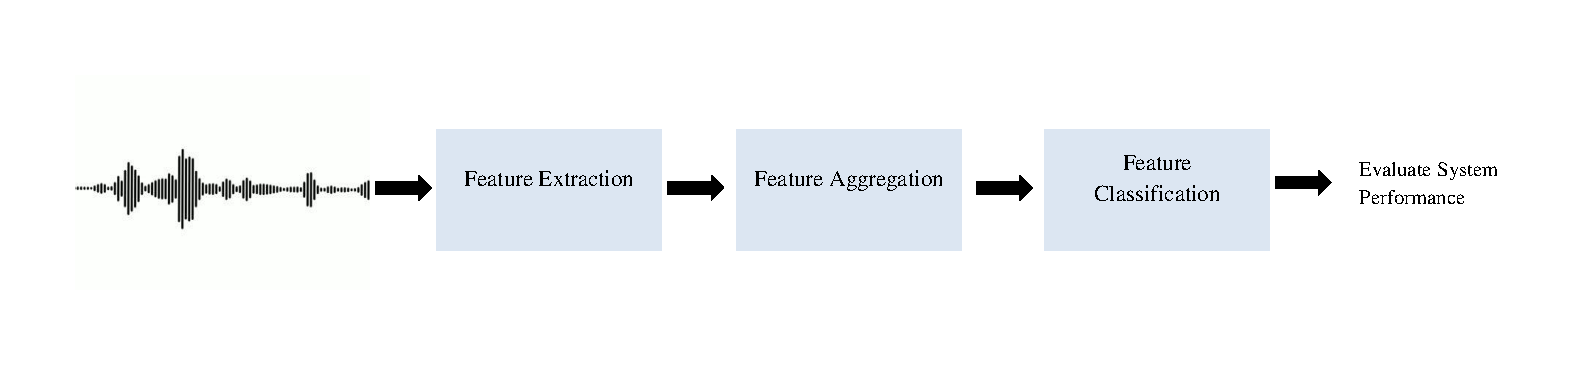
\includegraphics[scale=0.4]{Figures/pipeline.pdf}
  \end{center}
\caption{Pipeline of the genre classification system}
\end{figure}
  \begin{itemize}
    \item Learn features for a genre classification task using data from the GTZAN dataset.
    \item Train a classifier on the learned features and evaluate system performance.
    \item Inspect if features are general by using the same features on the ISMIR2004 genre dataset. 
  \end{itemize}  
\end{frame}

\begin{frame}{Contributions Of The Paper}
{\usebeamercolor[fg]{structure} Whats different?}
\begin{itemize}
    \item Evaluate the use of ReLUs as hidden units.
    \item Use Dropout for regularisation.
    \item Use HF Optimisation for training sigmoid nets and compare. 
  \end{itemize}
{\usebeamercolor[fg]{structure} Hypothesis?}
\begin{itemize}
    \item ReLUs+Dropout eliminate the need for pre-training.
    \item Performance(ReLU+Dropout+SGD) $>=$ Performance(sigmoid nets+SGD)
    \item More efficient training of sigmoid nets with HF.
  \end{itemize}
\end{frame}

\begin{frame}{Feature Extraction}
\begin{figure}
\begin{center}  
  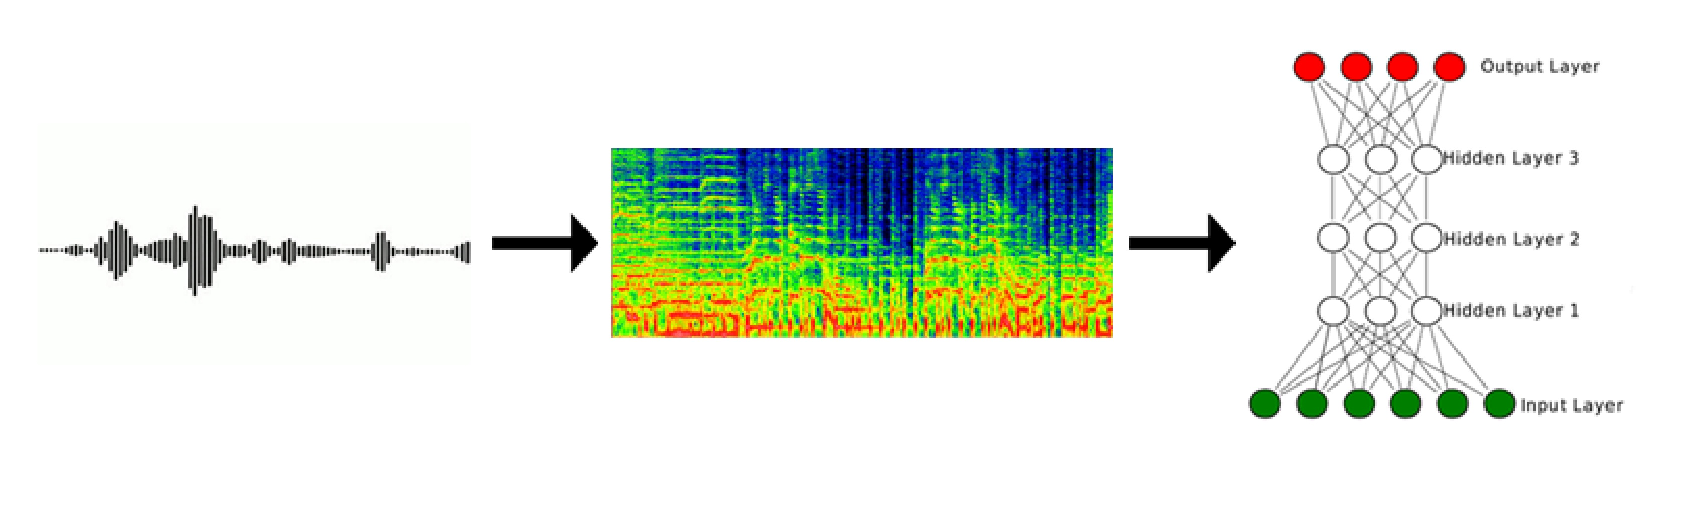
\includegraphics[scale=0.4]{Figures/feats.eps}
\end{center}
\caption{Feature extraction pipeline}
\end{figure}
\end{frame}

\begin{frame}{Rectified Linear Units}
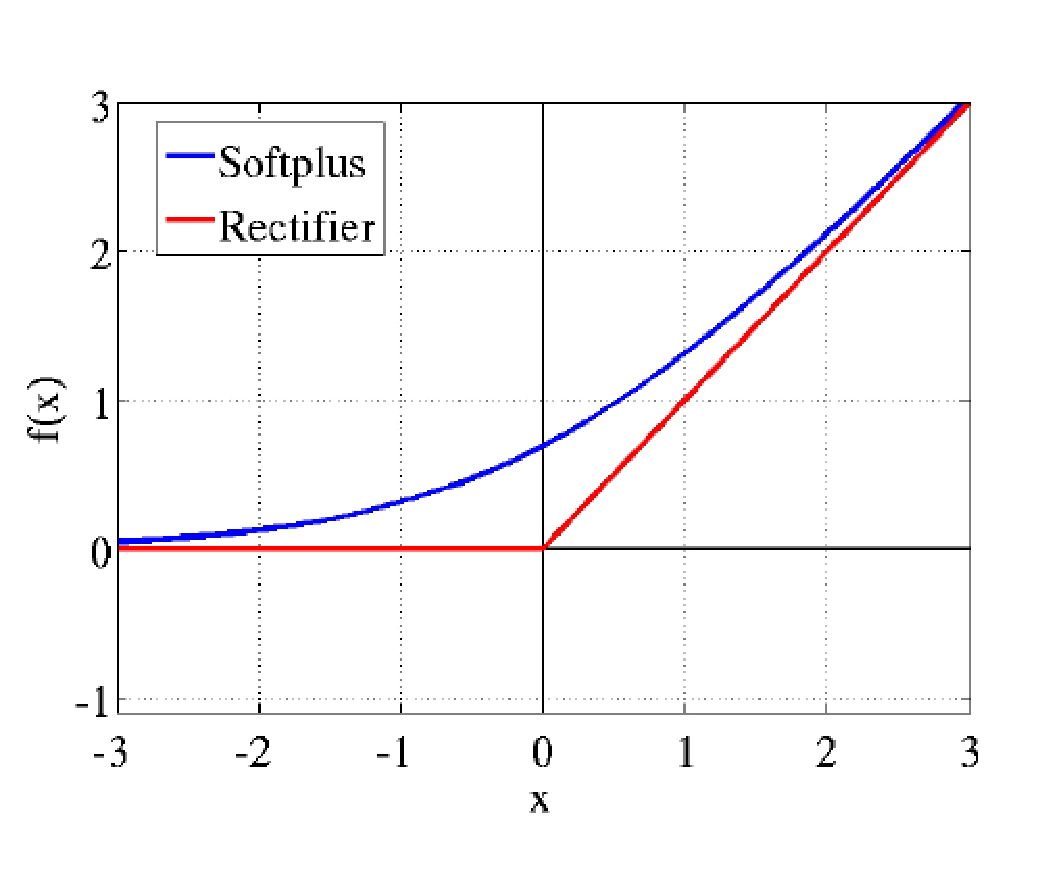
\includegraphics[width = .45\linewidth]{Figures/ReLU-acts.eps}
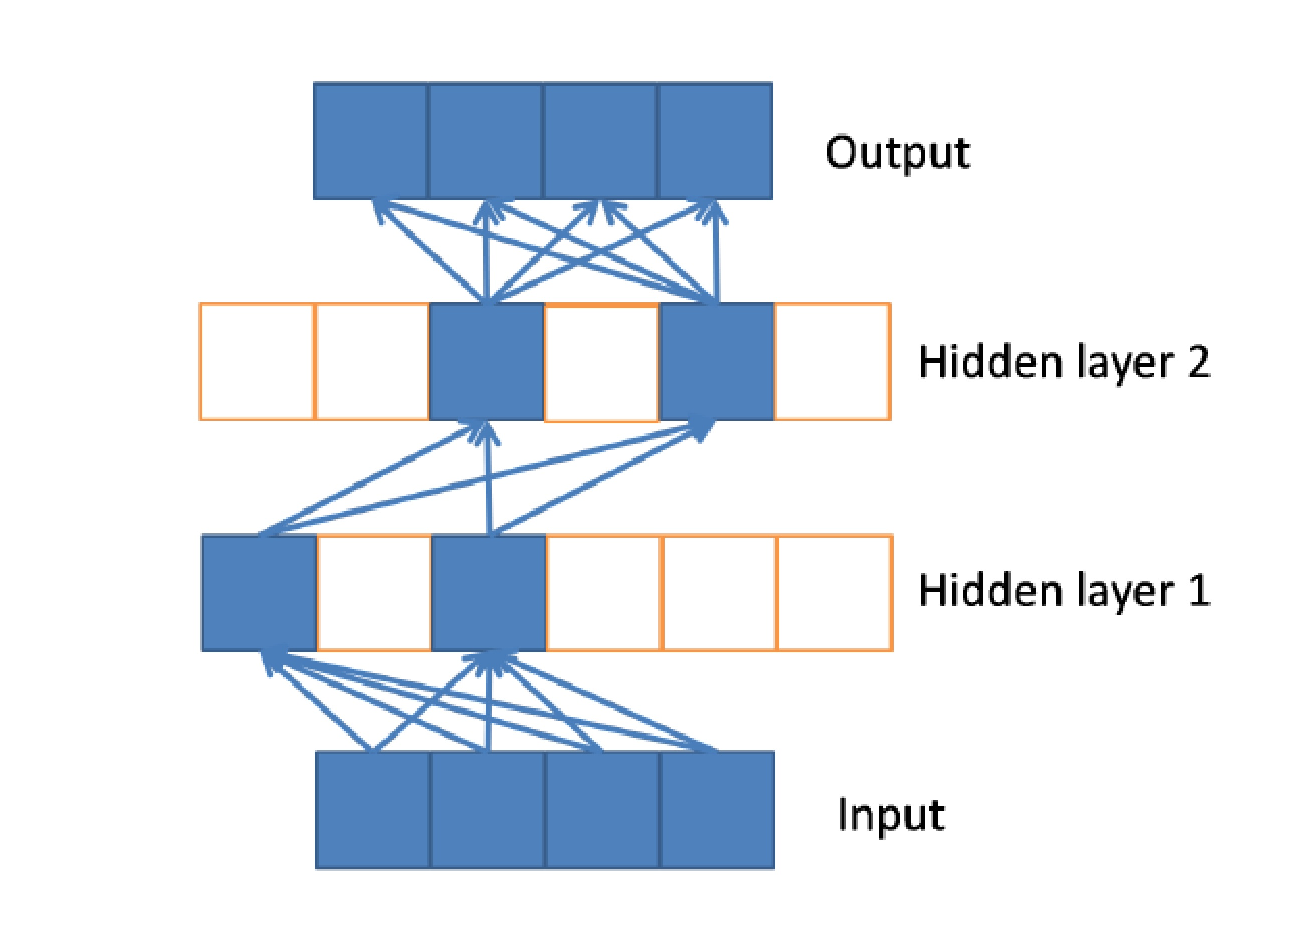
\includegraphics[width = .45\linewidth]{Figures/ReLU-grads.eps}
$$ \sum_{i}^{N} \sigma(x-i+0.5) \approx \log(1+e^{x})$$
\begin{center}
  NReLU: $ f(x) = max(0,x + \mathcal{N}(0,\sigma(x)))$\\
  ReLU: $f(x) = max(0,x) $
\end{center}
%\footnotetext[1]{Xavier Glorot, Antoine Bordes, and Yoshua Bengio. Deep sparse rectifier networks. In Proceedings of the 14th International Conference on Artificial Intelligence and Statistics. JMLR W&CP Volume, volume 15, pages 315–323, 2011}
\footnotetext[1]{Xavier Glorot, Antoine Bordes and Yoshua Bengio. Deep Sparse Rectifier Networks}
\end{frame}

\begin{frame}{Dropout}
\begin{figure}
\begin{center}  
  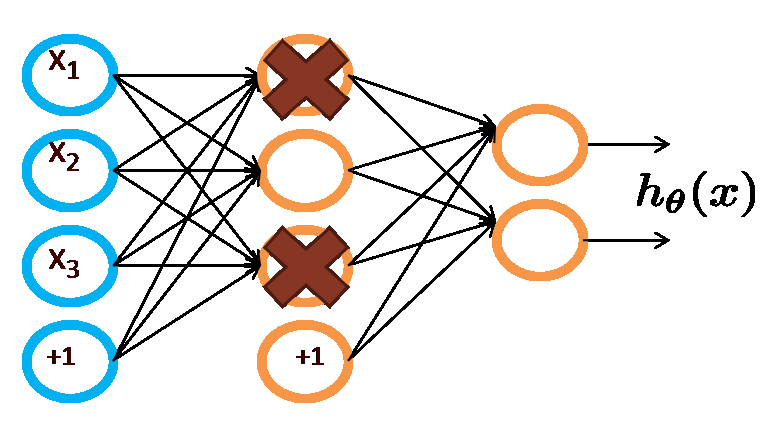
\includegraphics[scale=0.5]{Figures/dropout.eps}
\end{center}
\caption{Dropout: Some of the hidden units are masked during training}
\end{figure}
{\usebeamercolor[fg]{structure} Forward Propagation}
$$y^{l} = \frac{1}{1-p}W^{l}(r^{l-1} * y^{l-1} + b^{l})$$
\end{frame}

\begin{frame}{Useful Properties of ReLUs}
\begin{itemize}
    \item No need for supervised pre-training.
    \item Hard sparsity in hidden layers.
    \item Gradients flow easily.
    \item Error surface is less convoluted w.r.t parameters because of the form of the activation function.
  \end{itemize}
\end{frame}

\begin{frame}{Hessian Free Optimisation}
Newton's method: $ f(\theta_{n} + p) \approx f(\theta_{n}) + \nabla f(\theta_{n})^{T}p + \frac{1}{2}p^{T}Hp$\\
Newton's update: $\theta_{n+1} = \theta_{n} - H^{-1}\nabla f(p_{n})$\\
Quasi-newton use an approximation to the Hessian matrix $H$\\
Two main insights in HF:
\begin{itemize}
    \item The products $Hp$ can be easily calculated using finite derivatives. 
    \item The linear CG algorithm can be used to optimise the quadratic objective at each step. 
  \end{itemize}
\end{frame}

\begin{frame}{Datasets}

Tzanetakis Dataset:
\begin{itemize}
    \item 1000 examples, 30 seconds each, 22050 Hz.
    \item 10 genres. 
    \item 4, 50/25/25 train/valid/test splits. 
    \item Features aggregated over 5 seconds with a 2.5s overlap. 
  \end{itemize}
ISMIR 2004 Genre Dataset:
\begin{itemize}
    \item 1458 examples, truncated to 30 seconds each, downsampled to 22050 Hz.
    \item 6 genres. 
    \item Original test/train split. 
    \item Features aggregated over 5 seconds with a 2.5s overlap. 
  \end{itemize}
\end{frame}

\begin{frame}{Results: Tzanetakis Dataset}
 \begin{table} 
  \begin{center}
  \scalebox{0.8}{
  \begin{tabular}{ c | c | c | c | c}
    \hline
    &Hidden Units & ReLU+SGD & ReLU+SGD+Dropout &Sigmoid + HF\\ \hline
    &Layer 1 &75.0$\pm$1.7 & 76.5$\pm$1.5 &78.5$\pm$2.1\\ 
    50&Layer 2 & 79.6$\pm$2.7& 77.0$\pm$2.2 &80.0$\pm$2.6\\ 
    &Layer 3 &81.3$\pm$1.8& 78.0$\pm$1.0 &80.8$\pm$1.1\\ 
    &All &81.5$\pm$1.9& 81.5$\pm$1.7 &\textbf{82.1$\pm$1.7}\\ \hline
    &Layer 1 &71.8$\pm$0.7& 75.5$\pm$1.1 &67.8$\pm$1.5\\ 
    &Layer 2&79.5$\pm$1.9& 82.5$\pm$1.8 &74.0$\pm$2.6\\ 
    500&Layer 3&83.0$\pm$1.2& 82.0$\pm$1.4 &77.1$\pm$2.36\\ 
    &All&82.5$\pm$2.3 & \textbf{83.0$\pm$1.1}  &76.0$\pm$1.0\\ \hline
    \hline
  \end{tabular}}
  \end{center}
\caption{Genre classification results on the Tzanetakis dataset}
\end{table}  
\end{frame}

\begin{frame}{Results: ISMIR 2004 Dataset}
\begin{center}
\begin{table}
\scalebox{0.75}{
  \begin{tabular}{c| c | c | c | c}
    \hline
    Hidden Units & Layer & ReLU+SGD & ReLU+SGD+Dropout &Sigmoid + HF\\ \hline
    &1 & 70.50 & 68.03 &68.72\\ 
    50&2 & 70.80 & 66.94 &70.23\\ 
    &3 & 69.13& 68.03 &70.50\\ 
    &All & 72.42 & 69.68 &71.20\\ \hline
    &1 & 68.03 & 70.09 &68.40\\ 
    500&2 & 71.33 & 72.01 &68.32\\ 
    &3 & 71.46 & 69.41 &70.37\\ 
    &All & 72.30& \textbf{73.46} &70.23\\ \hline
    \hline
  \end{tabular}}
\caption{Genre classification results on the ISMIR 2004 dataset}
\vspace{-0.8em}
\end{table}  
\end{center}
\end{frame}

\begin{frame}{Observations}
\begin{itemize}
    \item Best accuracy is achieved with large hidden layers, ReLUs and Dropout.
    \item Classification accuracy is comparable to current state of the art with hand-crafted features. 
    \item Dropout does not work well for network with small number of hidden units. 
    \item HF achieves comparable results, though the ReLU performs better with large hidden layers. 
    \item The same features when used for the ISMIR dataset outperform MFCCs and PMSC features. 
\end{itemize}
\end{frame}

\begin{frame}{Conclusions}
\begin{itemize}
    \item ReLUs + SGD + Dropout learn good features are as effective as the state-of-the-art hand-crafted features.
    \item ReLU network learn good solutions without any pre-training. 
    \item HF is another attractive method for training neural nets. 
    \item The features learnt are general and can be reused for other tasks. 
\end{itemize}
\footnotetext[1]{Code:http://www.eecs.qmul.ac.uk/\~sss31/}
\end{frame}
\end{document}



